\documentclass[10pt, letterpaper, final]{article}
\usepackage[utf8]{inputenc}
\usepackage[T2A]{fontenc}
\usepackage[english,russian]{babel}
\usepackage{graphicx}
\graphicspath{{screens/}}
\usepackage{float}


\begin{document}
\title{s21\_SmartCalc V2.0 Description}
\author{Helper Carolee}
\date{May 2022}
\maketitle
\tolerance=10000
% \hspace{10pt}
  Программа s21\_smartcalc была разработана в рамках выполнения задания в Школе-21 Новосибирск. 
Вся логика программы разработана на языке Си++, графическая часть реализована на основе фреймворка Qt.
Основное окно программы представлено на рис \ref{fig:mesh1}.
Числовые значения с точкой и без, а так же знаки сложения , вычитания , деления  и умножения вводятся с числовой клавиатуры компьютера либо нажатием манипулятора "мышь" на соответсвующие изобрания клавишь на экране.
Ввод функций осуществляется только нажатием на виртуальные клавиши.
\begin{figure}[H]
   \centering
   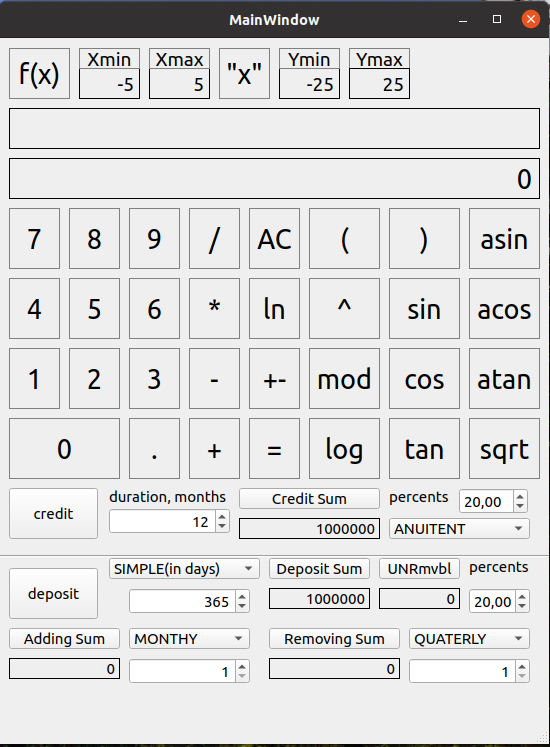
\includegraphics[width=0.6\textwidth]{base-window.png}
   \caption{основное окно калькулятора}
   \label{fig:mesh1}
\end{figure}

Для построения графика зависимости x от y необходимо вввести функцию зависимости f(x), при этом для введения Х в функцию надо нажимать символ Х вверху экранного блока. Для введения границ определения значений Х и У необходимо ввести их числовое значение и нажать соотвествующую кравишу на панели калькулятора в верхней его части. Для построени я графика необходимо нажать клавишу f(x), что приведет к открытию окна с построенным графиком функции, см. рис \ref{fig:mesh2}.

\begin{figure}[H]
%   \centering
   \center{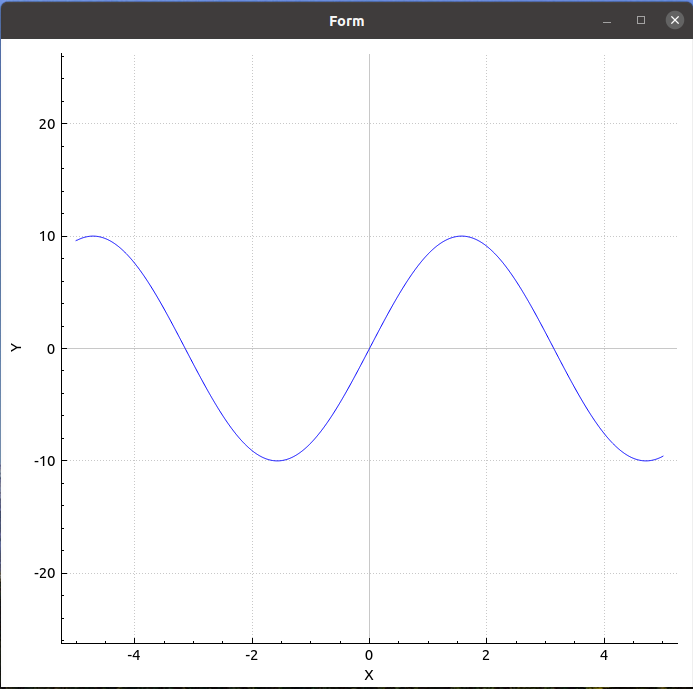
\includegraphics[width=1.0\textwidth]{xfunction-form.png}}
   \caption{график введенной функции}
   \label{fig:mesh2}
\end{figure}

\newpage
Для расчета кредита необходимо ввести размер желаемого кредита, срок его выплаты в месяцах и порядок платежей: ануитентный или регрессивный. Желательно учесть, что при ануитентой выплате суммарный размер процентов оказывается выше. После нажатия на кнопку на экран выводиться оно с расчетыми параметрами кредита - см. рис.\ref{fig:mesh3}.
%   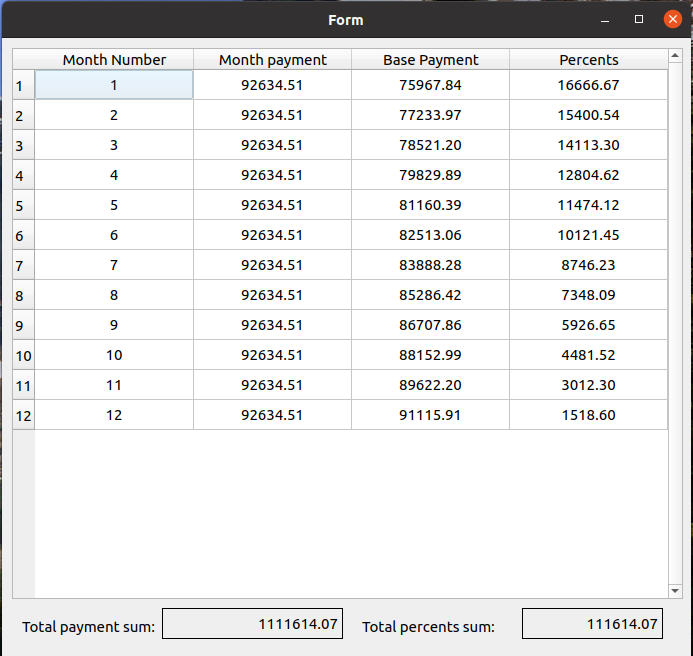
\includegraphics[width=0.5\textwidth]{credit-form.png}

\begin{figure}[H]
%   \centering
   \center{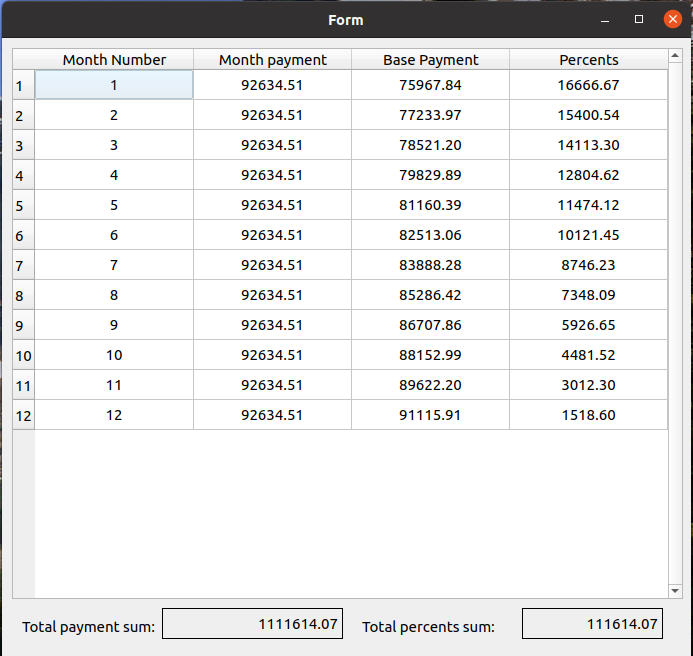
\includegraphics[width=1\textwidth]{credit-form.png}}
   \caption{кредитная таблица}
   \label{fig:mesh3}
\end{figure}
\newpage
Для расчета депозита необходимо заполнить параметры для дальнейшего расчета, при этом необходимо учитывать, что если выбран тип депозита SIMPLE, что частичных снятий и пополнений в расчете не будет.
после нажатия кнопки откроется окно с результатами расчета - см. рис.\ref{fig:mesh4}.

\begin{figure}[H]
%   \centering
   \center{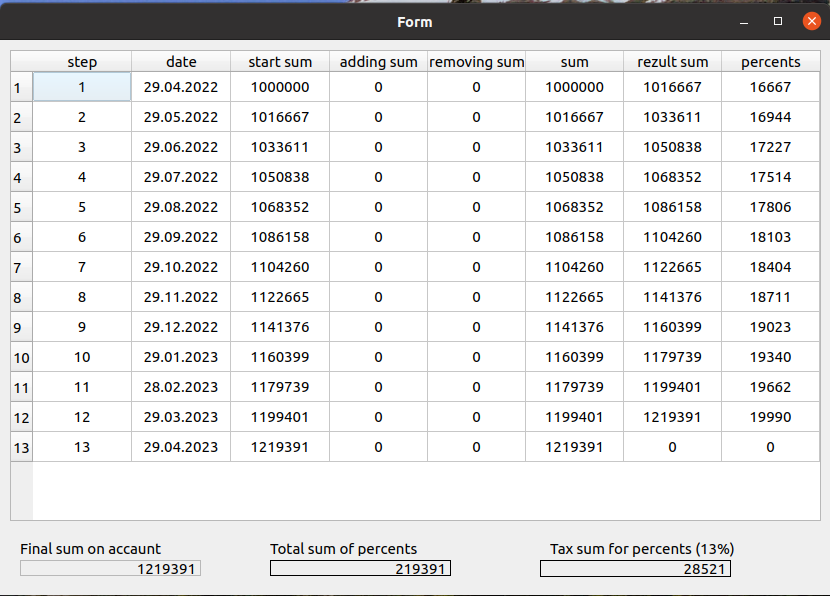
\includegraphics[width=1\textwidth]{deposit-form.png}}
   \caption{депозитная таблица}
   \label{fig:mesh4}
\end{figure}
В нижней части депозитной таблицы расположены значения итоговой суммы на счету клиента, Полной суммы уплаченных процентов, а так же размер требуемого к уплате налога с этих процентов. Напоминаю, что в 2021 и 2022 годах уплачивать налог с дохода по банковским вкладам согласно принятому в20 марта 2022 года закону не требуется. 
\end{document}
